\documentclass[12pt, a4paper]{article}

% ── Packages ──────────────────────────────────────────────────────────────────
\usepackage[a4paper, top=2.5cm, bottom=2.5cm, left=2.5cm, right=2.5cm, headheight=24.02pt]{geometry}
\usepackage[T1]{fontenc}
\usepackage[utf8]{inputenc}
\usepackage{mathptmx}          % Times New Roman font
\usepackage{amsmath}
\usepackage{amssymb}
\usepackage{pifont}
\usepackage{graphicx}
\usepackage{booktabs}
\usepackage{tabularx}
\usepackage{longtable}
\usepackage{array}
\usepackage{hyperref}
\usepackage{xcolor}
\usepackage{titlesec}
\usepackage{parskip}
\usepackage{enumitem}
\usepackage{fancyhdr}
\usepackage{caption}
\usepackage{subcaption}
\usepackage{float}
\usepackage{setspace}
\usepackage{tikz}
\usetikzlibrary{positioning,shapes.geometric,shapes.misc,arrows.meta}
\usepackage{mdframed}
\usepackage{tcolorbox}
\tcbuselibrary{skins, breakable}
\usepackage{acronym}           % For list of abbreviations
\usepackage{colortbl}
% References handled manually (IEEE-style numbered list in References section)
% Note: to cite inside text use \cite{} once you add a bibliography, or use [1], [2] notation manually

% ── Table formatting macros ───────────────────────────────────────────────────
\definecolor{tableheader}{RGB}{210, 225, 245}
\definecolor{tablerowalt}{RGB}{240, 244, 248}
\newcommand{\cellHigh}{\cellcolor{unigreen!25}}
\newcommand{\cellMed}{\cellcolor{accentgold!25}}
\newcommand{\cellLow}{\cellcolor{red!15}}
\newcommand{\theadrow}{\rowcolor{tableheader}}
\newcommand{\rowalt}{\rowcolor{tablerowalt}}
\newcommand{\crossmark}{\ding{55}}

% ── Colors ────────────────────────────────────────────────────────────────────
\definecolor{uniblue}{RGB}{0, 51, 102}
\definecolor{unigreen}{RGB}{34, 139, 34}
\definecolor{accentgold}{RGB}{180, 140, 0}
\definecolor{lightblue}{RGB}{235, 243, 255}
\definecolor{lightgray}{RGB}{245, 245, 245}
\definecolor{darkgray}{RGB}{80, 80, 80}
\definecolor{linkblue}{RGB}{52, 152, 219}
\definecolor{placeholdercolor}{RGB}{180, 0, 0}

% ── Placeholder command ───────────────────────────────────────────────────────
% Use  to mark inline placeholders
\newcommand{\TODO}[1]{\textcolor{placeholdercolor}{\textbf{[TODO: #1]}}}
% Use \TODOBLOCK{text} for multi-paragraph / list placeholder blocks
\newenvironment{TODOBLOCK}{%
  \begin{tcolorbox}[enhanced, colback=red!5, colframe=placeholdercolor,
    arc=2pt, boxrule=0.8pt, left=6pt, right=6pt, top=4pt, bottom=4pt,
    fonttitle=\small\bfseries, title={\textcolor{placeholdercolor}{TODO --- Fill in this section}}]
    \small\color{placeholdercolor}
}{%
  \end{tcolorbox}
}

% ── Hyperref ──────────────────────────────────────────────────────────────────
\hypersetup{
    colorlinks=true,
    linkcolor=uniblue,
    urlcolor=linkblue,
    pdftitle={CCI Department Choice Guidance System --- Industrial Practice Report},
    pdfauthor={Haramaya University CCI}
}

% ── Section heading styles ────────────────────────────────────────────────────
\titleformat{\section}
    {\large\bfseries\color{uniblue}}
    {\thesection.}{0.6em}{}
    [{\color{unigreen}\titlerule[1.5pt]}]
\titlespacing{\section}{0pt}{14pt}{6pt}

\titleformat{\subsection}
    {\normalsize\bfseries\color{uniblue}}
    {\thesubsection}{0.5em}{}
\titlespacing{\subsection}{0pt}{10pt}{4pt}

\titleformat{\subsubsection}
    {\normalsize\bfseries\color{darkgray}}
    {}{0em}{}
\titlespacing{\subsubsection}{0pt}{8pt}{2pt}

% ── Header / Footer ───────────────────────────────────────────────────────────
\pagestyle{fancy}
\fancyhf{}
\fancyhead[L]{\small\textcolor{uniblue}{\textbf{CCI Department Choice Guidance System}}}
\fancyhead[R]{\small\textcolor{uniblue}{Haramaya University --- CCI}}
\fancyfoot[C]{\textcolor{darkgray}{\thepage}}
\fancyfoot[L]{\small\textcolor{darkgray}{Industrial Practice Report}}
\fancyfoot[R]{\small\textcolor{darkgray}{June 2026}}
\renewcommand{\headrulewidth}{1pt}
\renewcommand{\footrulewidth}{0.4pt}
\renewcommand{\headrule}{\hbox to\headwidth{\color{uniblue}\leaders\hrule height \headrulewidth\hfill}}

\onehalfspacing

% ══════════════════════════════════════════════════════════════════════════════
\begin{document}
% ══════════════════════════════════════════════════════════════════════════════

% ─────────────────────────────────────────────────────────────────────────────
% PRELIMINARY 1: COVER PAGE
% ─────────────────────────────────────────────────────────────────────────────
\begin{titlepage}
\thispagestyle{empty}

\begin{tikzpicture}[remember picture, overlay]
    \draw[uniblue, line width=4pt]
        ([xshift=1cm, yshift=-1cm]current page.north west) --
        ([xshift=-1cm, yshift=-1cm]current page.north east);
    \draw[unigreen, line width=1.5pt]
        ([xshift=1cm, yshift=-1.4cm]current page.north west) --
        ([xshift=-1cm, yshift=-1.4cm]current page.north east);
    \draw[uniblue, line width=4pt]
        ([xshift=1cm, yshift=-1cm]current page.north west) --
        ([xshift=1cm, yshift=1cm]current page.south west);
    \draw[unigreen, line width=1.5pt]
        ([xshift=1.4cm, yshift=-1cm]current page.north west) --
        ([xshift=1.4cm, yshift=1cm]current page.south west);
    \draw[uniblue, line width=4pt]
        ([xshift=-1cm, yshift=-1cm]current page.north east) --
        ([xshift=-1cm, yshift=1cm]current page.south east);
    \draw[unigreen, line width=1.5pt]
        ([xshift=-1.4cm, yshift=-1cm]current page.north east) --
        ([xshift=-1.4cm, yshift=1cm]current page.south east);
    \draw[uniblue, line width=4pt]
        ([xshift=1cm, yshift=1cm]current page.south west) --
        ([xshift=-1cm, yshift=1cm]current page.south east);
    \draw[unigreen, line width=1.5pt]
        ([xshift=1cm, yshift=1.4cm]current page.south west) --
        ([xshift=-1cm, yshift=1.4cm]current page.south east);
    \node[anchor=south east] at ([xshift=-1.8cm, yshift=1.8cm]current page.south east) {
        \begin{tabular}{rl}
            \textbf{\textcolor{uniblue}{Submitted To:}} & Department of Computer Science\\[0.1cm]
            \textbf{\textcolor{uniblue}{Institution:}}  & Haramaya University\\[0.1cm]
            \textbf{\textcolor{uniblue}{Date:}}         & June 2026\\
        \end{tabular}
    };
\end{tikzpicture}

\begin{center}
\vspace*{0.5cm}

\includegraphics[width=3cm]{cci-logo.png}
\vspace{0.25cm}

{\large\bfseries\textcolor{uniblue}{YUUNIVARSIITII HARAMAAYAA}}\\[0.1cm]
{\Large\bfseries\textcolor{uniblue}{HARAMAYA UNIVERSITY}}\\[0.05cm]
{\small\itshape\textcolor{unigreen}{Building the Basis for Development}}\\[0.3cm]
{\normalsize\textcolor{darkgray}{College of Computing and Informatics}}\\[0.05cm]
{\normalsize\textcolor{darkgray}{Department of Computer Science}}\\[0.3cm]

{\color{uniblue}\rule{0.78\textwidth}{2.5pt}}\\[0.1cm]
{\color{unigreen}\rule{0.78\textwidth}{1pt}}\\[0.3cm]

\begin{tcolorbox}[
    enhanced, colback=uniblue, colframe=accentgold,
    arc=4pt, boxrule=1.5pt, width=0.82\textwidth,
    halign=center, top=10pt, bottom=10pt
]
    {\LARGE\bfseries\textcolor{white}{CCI DEPARTMENT CHOICE}}\\[2pt]
    {\LARGE\bfseries\textcolor{white}{GUIDANCE SYSTEM}}\\[6pt]
    {\normalsize\textcolor{white!80!gray}{Industrial Practice Report (Software Development)}}\\[3pt]
    {\small\textcolor{white!70!gray}{College of Computing and Informatics}}
\end{tcolorbox}

\vspace{0.2cm}
{\color{unigreen}\rule{0.78\textwidth}{1pt}}\\[0.08cm]
{\color{uniblue}\rule{0.78\textwidth}{2.5pt}}\\[0.3cm]

\begin{tcolorbox}[
    enhanced, colback=lightblue, colframe=uniblue,
    arc=4pt, boxrule=1pt, width=0.82\textwidth,
    top=6pt, bottom=6pt, left=10pt, right=10pt
]
\begin{flushleft}
{\bfseries\normalsize\textcolor{uniblue}{Group Members:}}\\[0.2cm]
\begin{tabular}{cll}
\textbf{\textcolor{uniblue}{No.}} & \textbf{\textcolor{uniblue}{Full Name}} & \textbf{\textcolor{uniblue}{ID Number}} \\[3pt]
\hline\\[-7pt]
1. & Asledin Abdukadir &  \\[2pt]
2. & Arafat Bule       &  \\[2pt]
3. & Burqa Jemal       &  \\[2pt]
4. & Usman Abdi        &  \\[2pt]
5. & Nuri Irko         &  \\[2pt]
\end{tabular}
\vspace{0.2cm}
\textcolor{uniblue}{\rule{0.70\textwidth}{0.5pt}}\\[0.15cm]
\begin{tabular}{ll}
\textbf{\textcolor{uniblue}{Advisor:}}     &  \\[2pt]
\textbf{\textcolor{uniblue}{Program:}}     &  \\[2pt]
\textbf{\textcolor{uniblue}{College:}}     & College of Computing and Informatics \\[2pt]
\textbf{\textcolor{uniblue}{Institution:}} & Haramaya University, Oromia, Ethiopia \\[2pt]
\textbf{\textcolor{uniblue}{Date:}}        & June 2026 \\[2pt]
\end{tabular}
\end{flushleft}
\end{tcolorbox}
\end{center}
\end{titlepage}

% ─────────────────────────────────────────────────────────────────────────────
% PRELIMINARY 2: ACKNOWLEDGEMENT
% ─────────────────────────────────────────────────────────────────────────────
\newpage
\thispagestyle{plain}
\section*{Acknowledgement}
\addcontentsline{toc}{section}{Acknowledgement}



\vspace{2cm}
\begin{flushright}
\textit{The Development Team}\\
\textit{College of Computing and Informatics}\\
\textit{Haramaya University}\\
\textit{June 2026}
\end{flushright}

% ─────────────────────────────────────────────────────────────────────────────
% PRELIMINARY 3: LIST OF ABBREVIATIONS
% ─────────────────────────────────────────────────────────────────────────────
\newpage
\section*{List of Abbreviations}
\addcontentsline{toc}{section}{List of Abbreviations}

\begin{acronym}[WCAG]  % longest acronym sets column width
  \acro{AI}    {Artificial Intelligence}
  \acro{API}   {Application Programming Interface}
  \acro{CCI}   {College of Computing and Informatics}
  \acro{CS}    {Computer Science}
  \acro{CSS}   {Cascading Style Sheets}
  \acro{DFD}   {Data Flow Diagram}
  \acro{FR}    {Functional Requirement}
  \acro{HOD}   {Head of Department}
  \acro{HTML}  {HyperText Markup Language}
  \acro{HTTP}  {HyperText Transfer Protocol}
  \acro{ICT}   {Information and Communication Technology}
  \acro{IS}    {Information System}
  \acro{ISC}   {Information Science}
  \acro{IT}    {Information Technology}
  \acro{JSON}  {JavaScript Object Notation}
  \acro{LLM}   {Large Language Model}
  \acro{MVC}   {Model-View-Controller}
  \acro{MVP}   {Minimum Viable Product}
  \acro{NFR}   {Non-Functional Requirement}
  \acro{NoSQL} {Not Only Structured Query Language}
  \acro{PDF}   {Portable Document Format}
  \acro{REST}  {Representational State Transfer}
  \acro{ROI}   {Return on Investment}
  \acro{STAT}  {Statistics}
  \acro{SWE}   {Software Engineering}
  \acro{TOC}   {Table of Contents}
  \acro{UI}    {User Interface}
  \acro{UX}    {User Experience}
  \acro{WBS}   {Work Breakdown Structure}
  \acro{WCAG}  {Web Content Accessibility Guidelines}
\end{acronym}

% ─────────────────────────────────────────────────────────────────────────────
% PRELIMINARY 4: TABLE OF CONTENTS
% ─────────────────────────────────────────────────────────────────────────────
\newpage
\tableofcontents
\newpage

% ─────────────────────────────────────────────────────────────────────────────
% PRELIMINARY 5: LIST OF TABLES AND FIGURES
% ─────────────────────────────────────────────────────────────────────────────
\listoftables
\addcontentsline{toc}{section}{List of Tables}
\newpage

\listoffigures
\addcontentsline{toc}{section}{List of Figures}
\newpage

% ─────────────────────────────────────────────────────────────────────────────
% PRELIMINARY 6: ORGANIZATION OF THE DOCUMENT
% ─────────────────────────────────────────────────────────────────────────────
\section*{Organization of the Document}
\addcontentsline{toc}{section}{Organization of the Document}

This report is organized into six chapters, each corresponding to a phase of the industrial practice, followed by appendices and references.

\begin{description}[leftmargin=2.5cm, style=nextline, itemsep=6pt]
\item[\textbf{Chapter 1 --- Introduction}]
    Provides background on Haramaya University and the College of Computing and Informatics (CCI), the organizational structure, team overview, project context, and the general and specific objectives of the industrial practice project.

\item[\textbf{Chapter 2 --- Software Development Plan}]
    Covers the project schedule with a Gantt chart, resource allocation, risk management strategy, development methodology (Agile), quality assurance plan, and the list of required documents to be produced.

\item[\textbf{Chapter 3 --- System Requirements}]
    Analyses the existing manual department-selection process and its limitations, then specifies the proposed system's functional requirements (what the system does) and non-functional requirements (performance, security, usability, and legal compliance).

\item[\textbf{Chapter 4 --- System Analysis \& Design}]
    Presents the system models including Data Flow Diagrams (Level 0, 1, and 2), the user interface design with screen mockups, the software architecture, and the security and access control design.

\item[\textbf{Chapter 5 --- Implementation}]
    Documents the development process, tools and technologies used, challenges encountered and how they were resolved, and the results of unit, integration, and system testing.

\item[\textbf{Chapter 6 --- Internship Reflection \& Conclusion}]
    Reflects on learning outcomes achieved during the internship, challenges faced in the workplace, and provides recommendations for the host organization and future internship programs.

\item[\textbf{Appendices}]
    Supplementary material including code snippets, full-size diagrams, survey questionnaire, and HOD interview template.

\item[\textbf{References}]
    All sources cited in IEEE format.
\end{description}

\clearpage

% ══════════════════════════════════════════════════════════════════════════════
%  CHAPTER 1: INTRODUCTION
% ══════════════════════════════════════════════════════════════════════════════
\section{Introduction}

% ─────────────────────────────────────────────────────────────────────────────
\subsection{Background of the Organization}
% ─────────────────────────────────────────────────────────────────────────────



% ─────────────────────────────────────────────────────────────────────────────
\subsection{Structure of the Organization}
% ─────────────────────────────────────────────────────────────────────────────



% ─────────────────────────────────────────────────────────────────────────────
\subsection{Team and Department Overview}
% ─────────────────────────────────────────────────────────────────────────────



The project team consists of five Computer Science students working under the supervision of the ICT Center:

\begin{table}[H]
\centering
\begin{tabularx}{\textwidth}{clXl}
\toprule
\theadrow
\textbf{No.} & \textbf{Name} & \textbf{Role \& Responsibilities} & \textbf{Contact} \\
\midrule
1 & Asledin Abdukadir & Project Manager / Backend Developer --- coordination, Express API, MongoDB, scoring algorithm &  \\[3pt]
\rowalt
2 & Arafat Bule & Frontend Lead --- React components, UI/UX implementation, responsive design &  \\[3pt]
3 & Burqa Jemal & Backend Developer --- LLM API integration, admin dashboard backend &  \\[3pt]
\rowalt
4 & Usman Abdi & Frontend Developer --- questionnaire UI, results visualization, PDF export &  \\[3pt]
5 & Nuri Irko & QA / Testing Lead --- test cases, user testing coordination, documentation &  \\
\bottomrule
\end{tabularx}
\caption{Development team roles and responsibilities}
\end{table}

% ─────────────────────────────────────────────────────────────────────────────
\subsection{Project Context}
% ─────────────────────────────────────────────────────────────────────────────

Each year approximately 400--500 new students join the College of Computing and Informatics (CCI) at Haramaya University and must choose one of six departments: Computer Science (CS), Software Engineering (SWE), Information Technology (IT), Information System (IS), Information Science (ISC), and Statistics (STAT). The selection occurs within the first 2--3 weeks of enrollment, yet no structured, Haramaya-specific guidance tool exists to support this decision.

A structured survey conducted with 43 current CCI students confirmed the problem: only 55.8\% felt fully confident they understood department differences, and 97.7\% indicated they would use or consider using a recommendation tool if one were available. Without adequate guidance, students risk mismatched placements that lead to dissatisfaction, department transfer requests, and in some cases delayed graduation.

The \textbf{CCI Department Choice Guidance System} is a web-based application developed to address this gap. It presents students with a structured 20--25 question assessment, applies a weighted scoring algorithm validated by department heads, and returns personalized department recommendations ranked by match percentage with AI-generated explanations.

\subsubsection*{Problem Statement}

\begin{tcolorbox}[
    enhanced, colback=lightblue, colframe=uniblue,
    arc=4pt, boxrule=1pt, top=6pt, bottom=6pt
]
\textit{``Incoming CCI students at Haramaya University lack a centralized, evidence-based tool to guide their department selection, resulting in uninformed choices, high transfer request rates, and student dissatisfaction.''}
\end{tcolorbox}

\subsubsection*{Project Scope Summary}

\begin{itemize}[leftmargin=1.5em, itemsep=3pt]
    \item \textbf{In scope}: Interactive assessment questionnaire, weighted recommendation engine, department information repository, admin content management dashboard, PDF export
    \item \textbf{Out of scope}: Native mobile apps, Amharic language support, integration with university registration system, video content, live chat support
    \item \textbf{Target users}: Incoming CCI students (primary), system administrators and HODs (secondary)
    \item \textbf{Deployment}: Web application hosted on Vercel (frontend) and Render (backend) with MongoDB Atlas database
\end{itemize}

% ─────────────────────────────────────────────────────────────────────────────
\subsection{Objectives}
% ─────────────────────────────────────────────────────────────────────────────

\subsubsection*{General Objective}

To design and develop a web-based department recommendation system that guides incoming CCI students at Haramaya University in making informed, evidence-based department selection decisions by providing personalized assessments, ranked recommendations, and comprehensive department information.

\subsubsection*{Specific Objectives}

\begin{enumerate}[leftmargin=1.5em, itemsep=4pt]
    \item Conduct a structured survey of current CCI students (target: $n \geq 40$) and HOD consultations to validate the problem and gather department-specific criteria data.
    \item Design and implement a 20--25 question interactive assessment questionnaire covering student interests, skills, career goals, and learning preferences.
    \item Develop a weighted scoring algorithm using HOD-validated criteria to compute match scores for all six CCI departments.
    \item Integrate an LLM API (OpenAI/Gemini) to generate personalized recommendation explanations, with template-based fallback.
    \item Build a department information repository with structured profiles for all six departments covering core focus, curriculum, career outcomes, and common misconceptions.
    \item Develop an administrative dashboard enabling authorized users to manage department content, review analytics, and update the question bank.
    \item Deploy the system to free-tier cloud infrastructure within the 6-week development timeline with 99\%+ uptime target.
    \item Achieve a minimum 70\% usage rate among incoming CCI students within the first enrollment period and 80\%+ user satisfaction rating.
\end{enumerate}

\clearpage

% ══════════════════════════════════════════════════════════════════════════════
%  CHAPTER 2: SOFTWARE DEVELOPMENT PLAN
% ══════════════════════════════════════════════════════════════════════════════
\section{Software Development Plan}

% ─────────────────────────────────────────────────────────────────────────────
\subsection{Project Schedule}
% ─────────────────────────────────────────────────────────────────────────────

The project follows a 6-week development timeline. The Gantt chart below visualizes phases, their durations, and the current status marker.

\begin{figure}[H]
\centering
\resizebox{\textwidth}{!}{%
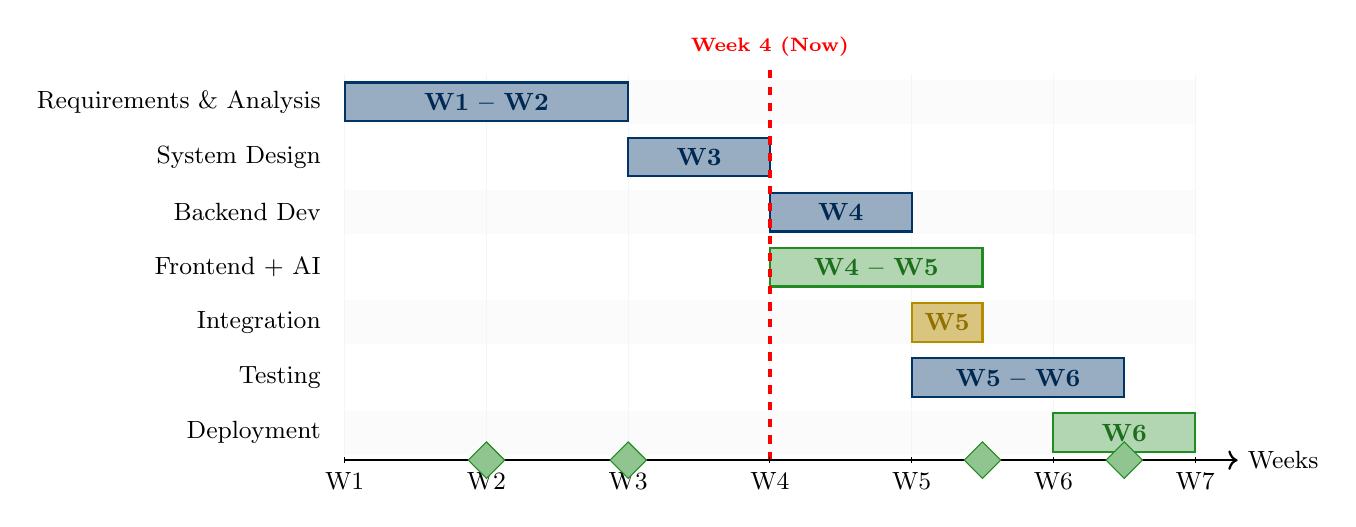
\begin{tikzpicture}[x=1.8cm, y=0.7cm]
\node[anchor=east, font=\small] at (0.9, 7) {Requirements \& Analysis};
\node[anchor=east, font=\small] at (0.9, 6) {System Design};
\node[anchor=east, font=\small] at (0.9, 5) {Backend Dev};
\node[anchor=east, font=\small] at (0.9, 4) {Frontend + AI};
\node[anchor=east, font=\small] at (0.9, 3) {Integration};
\node[anchor=east, font=\small] at (0.9, 2) {Testing};
\node[anchor=east, font=\small] at (0.9, 1) {Deployment};
\fill[lightgray!40] (1,6.6) rectangle (7,7.4);
\fill[lightgray!40] (1,4.6) rectangle (7,5.4);
\fill[lightgray!40] (1,2.6) rectangle (7,3.4);
\fill[lightgray!40] (1,0.6) rectangle (7,1.4);
\foreach \x in {1,2,...,7}
    \draw[lightgray, thin] (\x,0.5) -- (\x,7.5);
\fill[uniblue!40] (1,6.65) rectangle (3,7.35); \draw[uniblue,thick] (1,6.65) rectangle (3,7.35);
\node[font=\small\bfseries, text=uniblue!80!black] at (2,7) {W1 -- W2};
\fill[uniblue!40] (3,5.65) rectangle (4,6.35); \draw[uniblue,thick] (3,5.65) rectangle (4,6.35);
\node[font=\small\bfseries, text=uniblue!80!black] at (3.5,6) {W3};
\fill[uniblue!40] (4,4.65) rectangle (5,5.35); \draw[uniblue,thick] (4,4.65) rectangle (5,5.35);
\node[font=\small\bfseries, text=uniblue!80!black] at (4.5,5) {W4};
\fill[unigreen!35] (4,3.65) rectangle (5.5,4.35); \draw[unigreen,thick] (4,3.65) rectangle (5.5,4.35);
\node[font=\small\bfseries, text=unigreen!80!black] at (4.75,4) {W4 -- W5};
\fill[accentgold!50] (5,2.65) rectangle (5.5,3.35); \draw[accentgold,thick] (5,2.65) rectangle (5.5,3.35);
\node[font=\small\bfseries, text=accentgold!80!black] at (5.25,3) {W5};
\fill[uniblue!40] (5,1.65) rectangle (6.5,2.35); \draw[uniblue,thick] (5,1.65) rectangle (6.5,2.35);
\node[font=\small\bfseries, text=uniblue!80!black] at (5.75,2) {W5 -- W6};
\fill[unigreen!35] (6,0.65) rectangle (7,1.35); \draw[unigreen,thick] (6,0.65) rectangle (7,1.35);
\node[font=\small\bfseries, text=unigreen!80!black] at (6.5,1) {W6};
\draw[red, very thick, dashed] (4,0.5) -- (4,7.6);
\node[anchor=south, font=\scriptsize\bfseries, text=red] at (4,7.65) {Week 4 (Now)};
\draw[thick, ->] (1,0.5) -- (7.3,0.5) node[anchor=west, font=\small] {Weeks};
\foreach \x in {1,2,...,7}
    \draw (\x,0.55) -- (\x,0.45) node[anchor=north, font=\small] {W\x};
\node[diamond, draw=unigreen, fill=unigreen!50, minimum size=0.35cm] at (2,0.5) {};
\node[diamond, draw=unigreen, fill=unigreen!50, minimum size=0.35cm] at (3,0.5) {};
\node[diamond, draw=unigreen, fill=unigreen!50, minimum size=0.35cm] at (5.5,0.5) {};
\node[diamond, draw=unigreen, fill=unigreen!50, minimum size=0.35cm] at (6.5,0.5) {};
\end{tikzpicture}%
}
\caption{Project Gantt chart with milestones and current status}
\end{figure}

\begin{table}[H]
\centering
\begin{tabularx}{\textwidth}{p{3cm}p{2cm}Xc}
\toprule
\theadrow
\textbf{Milestone} & \textbf{Target Week} & \textbf{Critical Path Dependencies} & \textbf{Status} \\
\midrule
Project approval      & Week 1 & ICT Center endorsement; CCI Dean sign-off               & \cellHigh{}Done \\[3pt]
\rowalt
Requirements complete & Week 2 & Survey data collected; HOD responses (CS confirmed)      & \cellHigh{}Done \\[3pt]
Design approved       & Week 3 & Requirements finalized; architecture decisions made      & \cellHigh{}Done \\[3pt]
\rowalt
MVP ready             & Week 5 & Frontend + backend + LLM integration complete            & \cellMed{}In Progress \\[3pt]
Testing complete      & Week 6 & Beta testers recruited; major bugs resolved              & \cellMed{}Pending \\[3pt]
\rowalt
System deployed       & Week 6 & Hosting configured; handover documentation ready         & \cellMed{}Pending \\[3pt]
Live for enrollment   & Before June 1 & Operational before CCI enrollment period starts   & \cellMed{}Pending \\
\bottomrule
\end{tabularx}
\caption{Project milestone tracker}
\end{table}

% ─────────────────────────────────────────────────────────────────────────────
\subsection{Resources}
% ─────────────────────────────────────────────────────────────────────────────

\subsubsection*{Software Tools}

\begin{table}[H]
\centering
\begin{tabularx}{\textwidth}{p{3cm}p{3cm}X}
\toprule
\theadrow
\textbf{Tool / Technology} & \textbf{Category} & \textbf{Purpose} \\
\midrule
Electron           & Application shell      & Desktop runtime for the app; bundles HTML/CSS/JS into a desktop package \\[3pt]
\rowalt
HTML / CSS / JS    & Frontend               & Renderer UI, assessment flow, dashboard and PDF export logic (vanilla JS) \\[3pt]
Node.js / npm      & Build & Dependency management, packaging scripts, optional local tooling \\[3pt]
\rowalt
Chart.js (optional)& Visualization          & Charts used in the admin dashboard (optional) \\[3pt]
GitHub             & Version control        & Source code management, PRs, issues and CI \\[3pt]
\rowalt
MiKTeX / TeX Live   & Document build (local) & LaTeX toolchain used to compile the internship report PDF \\[3pt]
GitHub            & Version control      & Source code management, pull requests, code reviews \\[3pt]
\rowalt
VS Code            & IDE                    & Recommended editor; repo includes .vscode settings \\[3pt]
Figma              & UI/UX design           & Wireframes and prototype mockups \\[3pt]
\rowalt
Figma             & UI/UX design         & Wireframes and prototype mockups \\
\bottomrule
\end{tabularx}
\caption{Software tools and technologies used}
\end{table}

\subsubsection*{Hardware and Workspace}



\subsubsection*{Team Resource Allocation}

\begin{table}[H]
\centering
\begin{tabularx}{\textwidth}{p{3cm}p{3cm}Xc}
\toprule
\theadrow
\textbf{Team Member} & \textbf{Primary Role} & \textbf{Responsibilities} & \textbf{Allocation} \\
\midrule
Asledin Abdukadir & Project Manager / Backend Developer & Overall coordination, Express API, MongoDB integration, scoring algorithm & 100\% \\[3pt]
\rowalt
Arafat Bule & Frontend Lead & React components, UI/UX implementation, responsive design & 100\% \\[3pt]
Burqa Jemal & Backend Developer & LLM API integration, authentication, admin dashboard backend & 100\% \\[3pt]
\rowalt
Usman Abdi & Frontend Developer & Assessment questionnaire UI, results visualization, PDF export & 100\% \\[3pt]
Nuri Irko & QA / Testing Lead & Test case development, user testing coordination, documentation & 100\% \\[3pt]
\rowalt
ICT Center Supervisor & Technical Advisor & Weekly progress reviews, technical guidance, deployment approval & 10\% \\
\bottomrule
\end{tabularx}
\caption{Team resource allocation}
\end{table}

% ─────────────────────────────────────────────────────────────────────────────
\subsection{Risk Management}
% ─────────────────────────────────────────────────────────────────────────────

\begin{table}[H]
\centering
\begin{tabularx}{\textwidth}{p{3.5cm}ccp{6cm}}
\toprule
\theadrow
\textbf{Risk} & \textbf{Probability} & \textbf{Impact} & \textbf{Mitigation Strategy} \\
\midrule
Delayed HOD responses for all departments & High & Medium & Launch with CS data; add others incrementally; easy content update architecture \\[4pt]
\rowalt
Low student adoption rate & Medium & High & Integrate into orientation; promote via student leaders; beta test early \\[4pt]
LLM API quota exhaustion & Medium & Low & Caching; fallback templates; use Gemini (generous free tier) \\[4pt]
\rowalt
Timeline overruns & Low & Medium & Agile MVP focus; Week 6 buffer; prioritize core features \\[4pt]
Technical implementation challenges & Low & Medium & Proof-of-concept in Week 1; fallback to simpler solutions if needed \\[4pt]
\rowalt
Data privacy concerns & Low & Medium & Anonymous usage; 30-day auto-delete; clear privacy notice \\
\bottomrule
\end{tabularx}
\caption{Risk register with mitigation strategies}
\end{table}

% ─────────────────────────────────────────────────────────────────────────────
\subsection{Development Methodology}
% ─────────────────────────────────────────────────────────────────────────────

The project adopts an \textbf{Agile (Scrum-inspired)} methodology, justified by the following factors:

\begin{itemize}[leftmargin=1.5em, itemsep=3pt]
    \item \textbf{Short timeline}: 6-week development cycle favors iterative sprints (1-week each) over a sequential Waterfall approach that would compress testing to the very end.
    \item \textbf{Evolving requirements}: HOD content arrives incrementally; the system must be designed to accept new department data at any time without redesign.
    \item \textbf{Early feedback value}: Deploying an MVP by Week 5 and testing with real students before final delivery reduces the risk of building the wrong thing.
    \item \textbf{Team size}: A 5-member team maps well to Scrum roles (one product owner/PM, one Scrum master, three developers).
\end{itemize}

\textbf{Sprint structure} (1 week each):
\begin{enumerate}[leftmargin=1.5em, itemsep=2pt]
    \item \textbf{Week 1--2}: Requirements gathering, stakeholder interviews, architecture decisions
    \item \textbf{Week 3}: System design, database schema, API specification, UI wireframes
    \item \textbf{Week 4}: Backend core (Express API, MongoDB, scoring engine)
    \item \textbf{Week 4--5}: Frontend build (React UI, questionnaire, results page) + LLM integration
    \item \textbf{Week 5}: Integration sprint (connect all layers, smoke test)
    \item \textbf{Week 6}: Testing, bug fixes, deployment, documentation handover
\end{enumerate}

\textbf{Communication cadence}:
\begin{table}[H]
\centering
\begin{tabularx}{\textwidth}{p{3cm}p{2.5cm}Xp{2.5cm}}
\toprule
\theadrow
\textbf{Meeting Type} & \textbf{Frequency} & \textbf{Participants} & \textbf{Purpose} \\
\midrule
Daily standup        & Daily, 15 min       & Development team                  & Progress, blockers, coordination \\[3pt]
\rowalt
Sprint planning      & Weekly, 1 hr        & Development team                  & Define deliverables, assign tasks \\[3pt]
ICT Center check-in  & Weekly, 30 min      & Team lead + ICT supervisor        & Progress review, guidance \\[3pt]
\rowalt
Stakeholder update   & Bi-weekly, 30 min   & Team lead + CCI Dean / HODs       & Status, content review, feedback \\[3pt]
Retrospective        & End of project      & Development team                  & Lessons learned, documentation \\
\bottomrule
\end{tabularx}
\caption{Communication and meeting schedule}
\end{table}

% ─────────────────────────────────────────────────────────────────────────────
\subsection{Quality Assurance}
% ─────────────────────────────────────────────────────────────────────────────

\begin{itemize}[leftmargin=1.5em, itemsep=3pt]
    \item \textbf{Code reviews}: All code merged via GitHub pull requests with at least one peer reviewer before merging to main branch
    \item \textbf{Automated testing}: Unit tests for scoring algorithm and API endpoints targeting 80\% code coverage (Jest framework)
    \item \textbf{Manual testing}: Comprehensive test cases for all user workflows documented in a test matrix
    \item \textbf{User acceptance testing (UAT)}: 10--15 beta testers representing different CCI departments and backgrounds; structured feedback form
    \item \textbf{Performance testing}: Load test with 50 simulated concurrent users using Apache JMeter
    \item \textbf{Accessibility testing}: WCAG 2.1 Level AA compliance verification using automated tools (axe-core) plus manual keyboard navigation testing
    \item \textbf{Documentation standards}: JSDoc for all API functions; README for each major module; inline comments for complex logic
\end{itemize}

% ─────────────────────────────────────────────────────────────────────────────
\subsection{Required Documents}
% ─────────────────────────────────────────────────────────────────────────────

\begin{table}[H]
\centering
\begin{tabularx}{\textwidth}{p{4cm}Xc}
\toprule
\theadrow
\textbf{Document} & \textbf{Content Summary} & \textbf{Target Week} \\
\midrule
Requirements Specification & Functional requirements, non-functional requirements, user stories, acceptance criteria & Week 2 \\[3pt]
\rowalt
System Design Document     & Architecture diagrams, database schema, API specifications, UI/UX mockups & Week 3 \\[3pt]
User Guide (Students)      & Step-by-step instructions for assessment, results interpretation, comparison tool & Week 6 \\[3pt]
\rowalt
Administrator Manual       & Content management procedures, analytics, system maintenance & Week 6 \\[3pt]
Technical Documentation    & Codebase overview, deployment instructions, API reference, troubleshooting & Week 6 \\[3pt]
\rowalt
Handover Report            & Architecture decisions, maintenance recommendations, contact information & Week 6 \\[3pt]
Industrial Practice Report & This document --- complete report as per CCI guideline & Week 6 \\
\bottomrule
\end{tabularx}
\caption{Required project documents and delivery schedule}
\end{table}

\clearpage

% ══════════════════════════════════════════════════════════════════════════════
%  CHAPTER 3: SYSTEM REQUIREMENTS
% ══════════════════════════════════════════════════════════════════════════════
\section{System Requirements}

% ─────────────────────────────────────────────────────────────────────────────
\subsection{Existing System Analysis}
% ─────────────────────────────────────────────────────────────────────────────

\subsubsection*{Overview of the Current Process}

The current department selection process at CCI operates entirely through informal channels:

\begin{itemize}[leftmargin=1.5em, itemsep=3pt]
    \item Students receive general orientation materials describing departments in broad terms
    \item Department heads present at orientation sessions (typically 15--20 minutes per department)
    \item Students consult seniors, family members, or general internet sources
    \item Final selection is made within the first 2--3 weeks of enrollment
    \item No structured individual assessment of student interests, skills, or career goals exists
    \item No centralized, Haramaya-specific information repository is available
\end{itemize}

\subsubsection*{Limitations of the Existing System}

A structured survey of 43 current CCI students revealed the following measurable limitations:

\begin{table}[H]
\centering
\begin{tabularx}{\textwidth}{p{4cm}Xp{2cm}}
\toprule
\theadrow
\textbf{Limitation} & \textbf{Evidence} & \textbf{Impact} \\
\midrule
No personalized guidance & 44.2\% of students felt uncertain about differences between departments & High \\[4pt]
\rowalt
No centralized resource & Students rely on WhatsApp rumors and senior opinions & Medium \\[4pt]
No misconception correction & CS HOD noted students consistently underestimate department's creative demands & Medium \\[4pt]
\rowalt
High transfer rate & Registrar reports 15--20\% first-year transfer request rate (anecdotal) & High \\[4pt]
Enrollment imbalance & Some departments over-enrolled; others under-enrolled despite job market demand & Medium \\
\bottomrule
\end{tabularx}
\caption{Limitations of the current department selection process}
\end{table}

% ─────────────────────────────────────────────────────────────────────────────
\subsection{Proposed System}
% ─────────────────────────────────────────────────────────────────────────────

\subsubsection*{Functional Requirements}

\begin{table}[H]
\centering
\begin{tabularx}{\textwidth}{p{1.2cm}p{3.5cm}X}
\toprule
\theadrow
\textbf{ID} & \textbf{Feature} & \textbf{Description} \\
\midrule
FR-01 & Assessment questionnaire & The system shall present 20--25 questions one at a time with a progress indicator and support forward/backward navigation \\[4pt]
\rowalt
FR-02 & Response auto-save & The system shall auto-save the student's progress after each answer so it can be resumed if interrupted \\[4pt]
FR-03 & Match score computation & The system shall compute a match score (0--100) for all six departments using a weighted algorithm and complete within 3 seconds \\[4pt]
\rowalt
FR-04 & Department ranking & The system shall rank all six departments by match score and select the top 3 for detailed display \\[4pt]
FR-05 & AI explanation generation & The system shall invoke an LLM API to generate a personalized explanation for each recommendation with a 5-second timeout and template fallback \\[4pt]
\rowalt
FR-06 & Results display & The system shall display the top 3 departments with match percentages, visual progress bars, personalized text, and action buttons (Learn More, Compare, Download PDF) \\[4pt]
FR-07 & Department comparison & The system shall allow students to select 2--4 departments and display a side-by-side comparison table exportable as PDF \\[4pt]
\rowalt
FR-08 & Admin authentication & The system shall require username + password authentication for admin access with bcrypt hashing and 30-minute session timeout \\[4pt]
FR-09 & Content management & Authenticated admins shall be able to create, update, and delete department profiles and assessment questions via a structured form interface \\[4pt]
\rowalt
FR-10 & Audit trail & The system shall log all content changes with timestamp and admin ID and allow rollback to previous versions \\[4pt]
FR-11 & Analytics dashboard & The admin dashboard shall display usage statistics, recommendation distribution by department, and aggregated feedback ratings \\[4pt]
\rowalt
FR-12 & CSV export & Administrators shall be able to export analytics data as CSV for offline reporting \\
\bottomrule
\end{tabularx}
\caption{Functional requirements}
\end{table}

\subsubsection*{Non-Functional Requirements}



\begin{table}[H]
\centering
\begin{tabularx}{\textwidth}{p{1.2cm}p{3cm}Xp{2.5cm}}
\toprule
\theadrow
\textbf{ID} & \textbf{Category} & \textbf{Requirement} & \textbf{Measure / Target} \\
\midrule
NFR-01 & \textbf{Performance}    & The system shall generate recommendation results within 3 seconds of assessment completion under normal load & $\leq 3$ seconds \\[4pt]
\rowalt
NFR-02 & \textbf{Performance}    & The system shall support at least 50 concurrent users without degradation & 50 concurrent users \\[4pt]
NFR-03 & \textbf{Reliability}    & The system shall maintain 99\%+ uptime during the CCI enrollment period (June--August) & $\geq 99\%$ uptime \\[4pt]
\rowalt
NFR-04 & \textbf{Usability}      & A first-time user with no training shall be able to complete the full assessment without external help & Zero-training target \\[4pt]
NFR-05 & \textbf{Usability}      & The system shall be fully functional on screen widths from 320px (mobile) to 1920px (desktop) & Responsive 320--1920px \\[4pt]
\rowalt
NFR-06 & \textbf{Accessibility}  & The system shall comply with WCAG 2.1 Level AA standards & WCAG 2.1 AA \\[4pt]
NFR-07 & \textbf{Security}       & Student response data shall be stored anonymously with no personal identifiers & No PII stored \\[4pt]
\rowalt
NFR-08 & \textbf{Security}       & All student response data shall be automatically deleted after 30 days & 30-day auto-delete \\[4pt]
NFR-09 & \textbf{Security}       & Admin passwords shall be hashed using bcrypt with a minimum cost factor of 12 & bcrypt cost $\geq 12$ \\[4pt]
\rowalt
NFR-10 & \textbf{Security}       & All API communication shall use HTTPS & HTTPS enforced \\[4pt]
NFR-11 & \textbf{Maintainability}& The codebase shall achieve $\geq 80\%$ unit test coverage on the scoring algorithm and API endpoints & $\geq 80\%$ coverage \\[4pt]
\rowalt
NFR-12 & \textbf{Legal}          & The system shall comply with applicable Ethiopian data privacy guidelines and the university's data retention policy & Full compliance \\[4pt]
NFR-13 & \textbf{Scalability}    & Adding a new department profile shall require only a database update with no code changes & Zero-code department addition \\
\bottomrule
\end{tabularx}
\caption{Non-functional requirements}
\end{table}

\clearpage

% ══════════════════════════════════════════════════════════════════════════════
%  CHAPTER 4: SYSTEM ANALYSIS & DESIGN
% ══════════════════════════════════════════════════════════════════════════════
\section{System Analysis and Design}

% ─────────────────────────────────────────────────────────────────────────────
\subsection{System Models}
% ─────────────────────────────────────────────────────────────────────────────

\subsubsection*{Use Case Diagram}



\subsubsection*{Class / Object Diagram}



\subsubsection*{Activity / Sequence Diagram --- Student Assessment Flow}

The following activity diagram models the complete student journey through the assessment and recommendation process.

\begin{figure}[H]
\centering
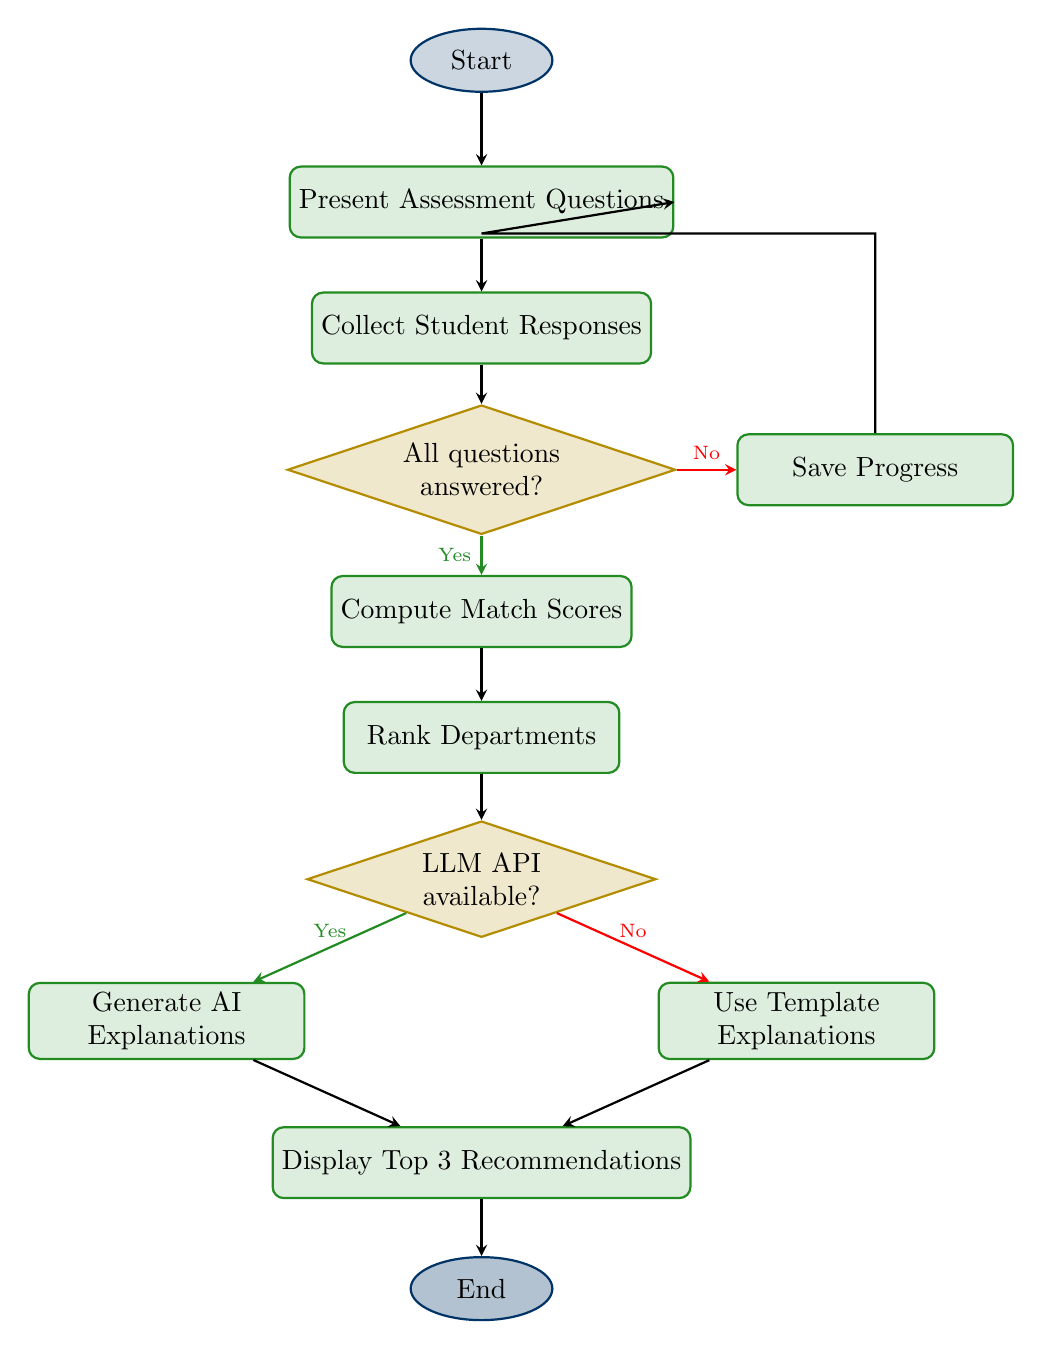
\begin{tikzpicture}[
    start/.style={ellipse, draw=uniblue, fill=uniblue!20, thick, minimum width=1.8cm, minimum height=0.8cm, align=center},
    proc/.style={rectangle, draw=unigreen, fill=unigreen!15, thick, minimum width=3.5cm, minimum height=0.9cm, align=center, rounded corners},
    dec/.style={diamond, draw=accentgold, fill=accentgold!20, thick, minimum width=1.8cm, align=center, aspect=3},
    endst/.style={ellipse, draw=uniblue, fill=uniblue!30, thick, minimum width=1.8cm, minimum height=0.8cm, align=center},
    arrow/.style={->, thick, >=stealth}
]
% Main flow (centred at x=0)
\node[start]  at (0, 0)    (start)   {Start};
\node[proc]   at (0,-1.8)  (present) {Present Assessment Questions};
\node[proc]   at (0,-3.4)  (collect) {Collect Student Responses};
\node[dec]    at (0,-5.2)  (complete){All questions\\answered?};
\node[proc]   at (0,-7)    (compute) {Compute Match Scores};
\node[proc]   at (0,-8.6)  (rank)    {Rank Departments};
\node[dec]    at (0,-10.4) (llm)     {LLM API\\available?};
\node[proc]   at (-4,-12.2)(generate){Generate AI\\Explanations};
\node[proc]   at ( 4,-12.2)(template){Use Template\\Explanations};
\node[proc]   at (0,-14)   (display) {Display Top 3 Recommendations};
\node[endst]  at (0,-15.6) (end)     {End};
% Save progress branch (right side)
\node[proc]   at (5,-5.2)  (save)    {Save Progress};

\draw[arrow] (start)    -- (present);
\draw[arrow] (present)  -- (collect);
\draw[arrow] (collect)  -- (complete);
\draw[arrow, color=unigreen] (complete) -- node[left,font=\scriptsize]  {Yes} (compute);
\draw[arrow, color=red]      (complete) -- node[above,font=\scriptsize] {No}  (save);
\draw[arrow] (save) -- ++(0,3) -- ++(-5,0) -- (present.east);
\draw[arrow] (compute)  -- (rank);
\draw[arrow] (rank)     -- (llm);
\draw[arrow, color=unigreen] (llm)  -- node[above,font=\scriptsize] {Yes} (generate);
\draw[arrow, color=red]      (llm)  -- node[above,font=\scriptsize] {No}  (template);
\draw[arrow] (generate) -- (display);
\draw[arrow] (template) -- (display);
\draw[arrow] (display)  -- (end);
\end{tikzpicture}
\caption{Activity diagram --- student assessment and recommendation flow}
\end{figure}



\subsubsection*{Data Flow Diagrams}

\paragraph{Level 0 DFD (Context Diagram)}

\begin{figure}[H]
\centering
\resizebox{0.85\textwidth}{!}{%
\begin{tikzpicture}[
    entity/.style={rectangle, draw=uniblue, thick, fill=lightblue, minimum width=3cm, minimum height=1.1cm, align=center, font=\small},
    process/.style={circle, draw=unigreen, fill=unigreen!20, thick, minimum size=3.6cm, align=center, font=\bfseries\small},
    inp/.style={->, thick, >=stealth, uniblue},
    outarrow/.style={->, thick, >=stealth, dashed, darkgray}
]
\node[process, text width=3cm] (system) at (0,0) {\textbf{0}\\[-2pt]CCI Dept\\Choice\\Guidance\\System};
\node[entity, text width=2.8cm] (student) at (-6.5, 0)  {Prospective\\Student};
\node[entity, text width=2.8cm] (admin)   at ( 6.5, 0)  {System\\Administrator};
\node[entity, text width=2.8cm] (hod)     at ( 0,  -5)  {Department\\Head};
\node[entity, text width=2.8cm] (llm)     at ( 0,   5)  {LLM API\\(OpenAI/Gemini)};
\draw[inp] ([yshift=8pt]student.east) -- ([yshift=8pt]system.west)
    node[midway, above, font=\footnotesize] {Student responses};
\draw[outarrow] ([yshift=-8pt]system.west) -- ([yshift=-8pt]student.east)
    node[midway, below, font=\footnotesize, text width=2.6cm, align=center] {Personalized recommendations};
\draw[inp] ([yshift=8pt]admin.west) -- ([yshift=8pt]system.east)
    node[midway, above, font=\footnotesize, text width=2.4cm, align=center] {Content updates, Config changes};
\draw[outarrow] ([yshift=-8pt]system.east) -- ([yshift=-8pt]admin.west)
    node[midway, below, font=\footnotesize, text width=2cm, align=center] {Analytics, Usage stats};
\draw[inp] ([xshift=8pt]hod.north) -- ([xshift=8pt]system.south)
    node[midway, right, font=\footnotesize, text width=2.2cm, align=left] {Dept profiles,\\Criteria weights};
\draw[out] ([xshift=-8pt]system.south) -- ([xshift=-8pt]hod.north)
    node[midway, left, font=\footnotesize, text width=2.4cm, align=right] {Student feedback,\\Enrollment data};
\draw[inp] ([xshift=-8pt]llm.south) -- ([xshift=-8pt]system.north)
    node[midway, left, font=\footnotesize, text width=2cm, align=right] {AI-generated\\explanations};
\draw[out] ([xshift=8pt]system.north) -- ([xshift=8pt]llm.south)
    node[midway, right, font=\footnotesize, text width=2.5cm, align=left] {Explanation\\generation request};
\end{tikzpicture}%
}
\caption{Level 0 DFD --- system context diagram}
\end{figure}

\paragraph{Level 1 DFD (Major Processes)}

\begin{figure}[H]
\centering
\resizebox{\textwidth}{!}{%
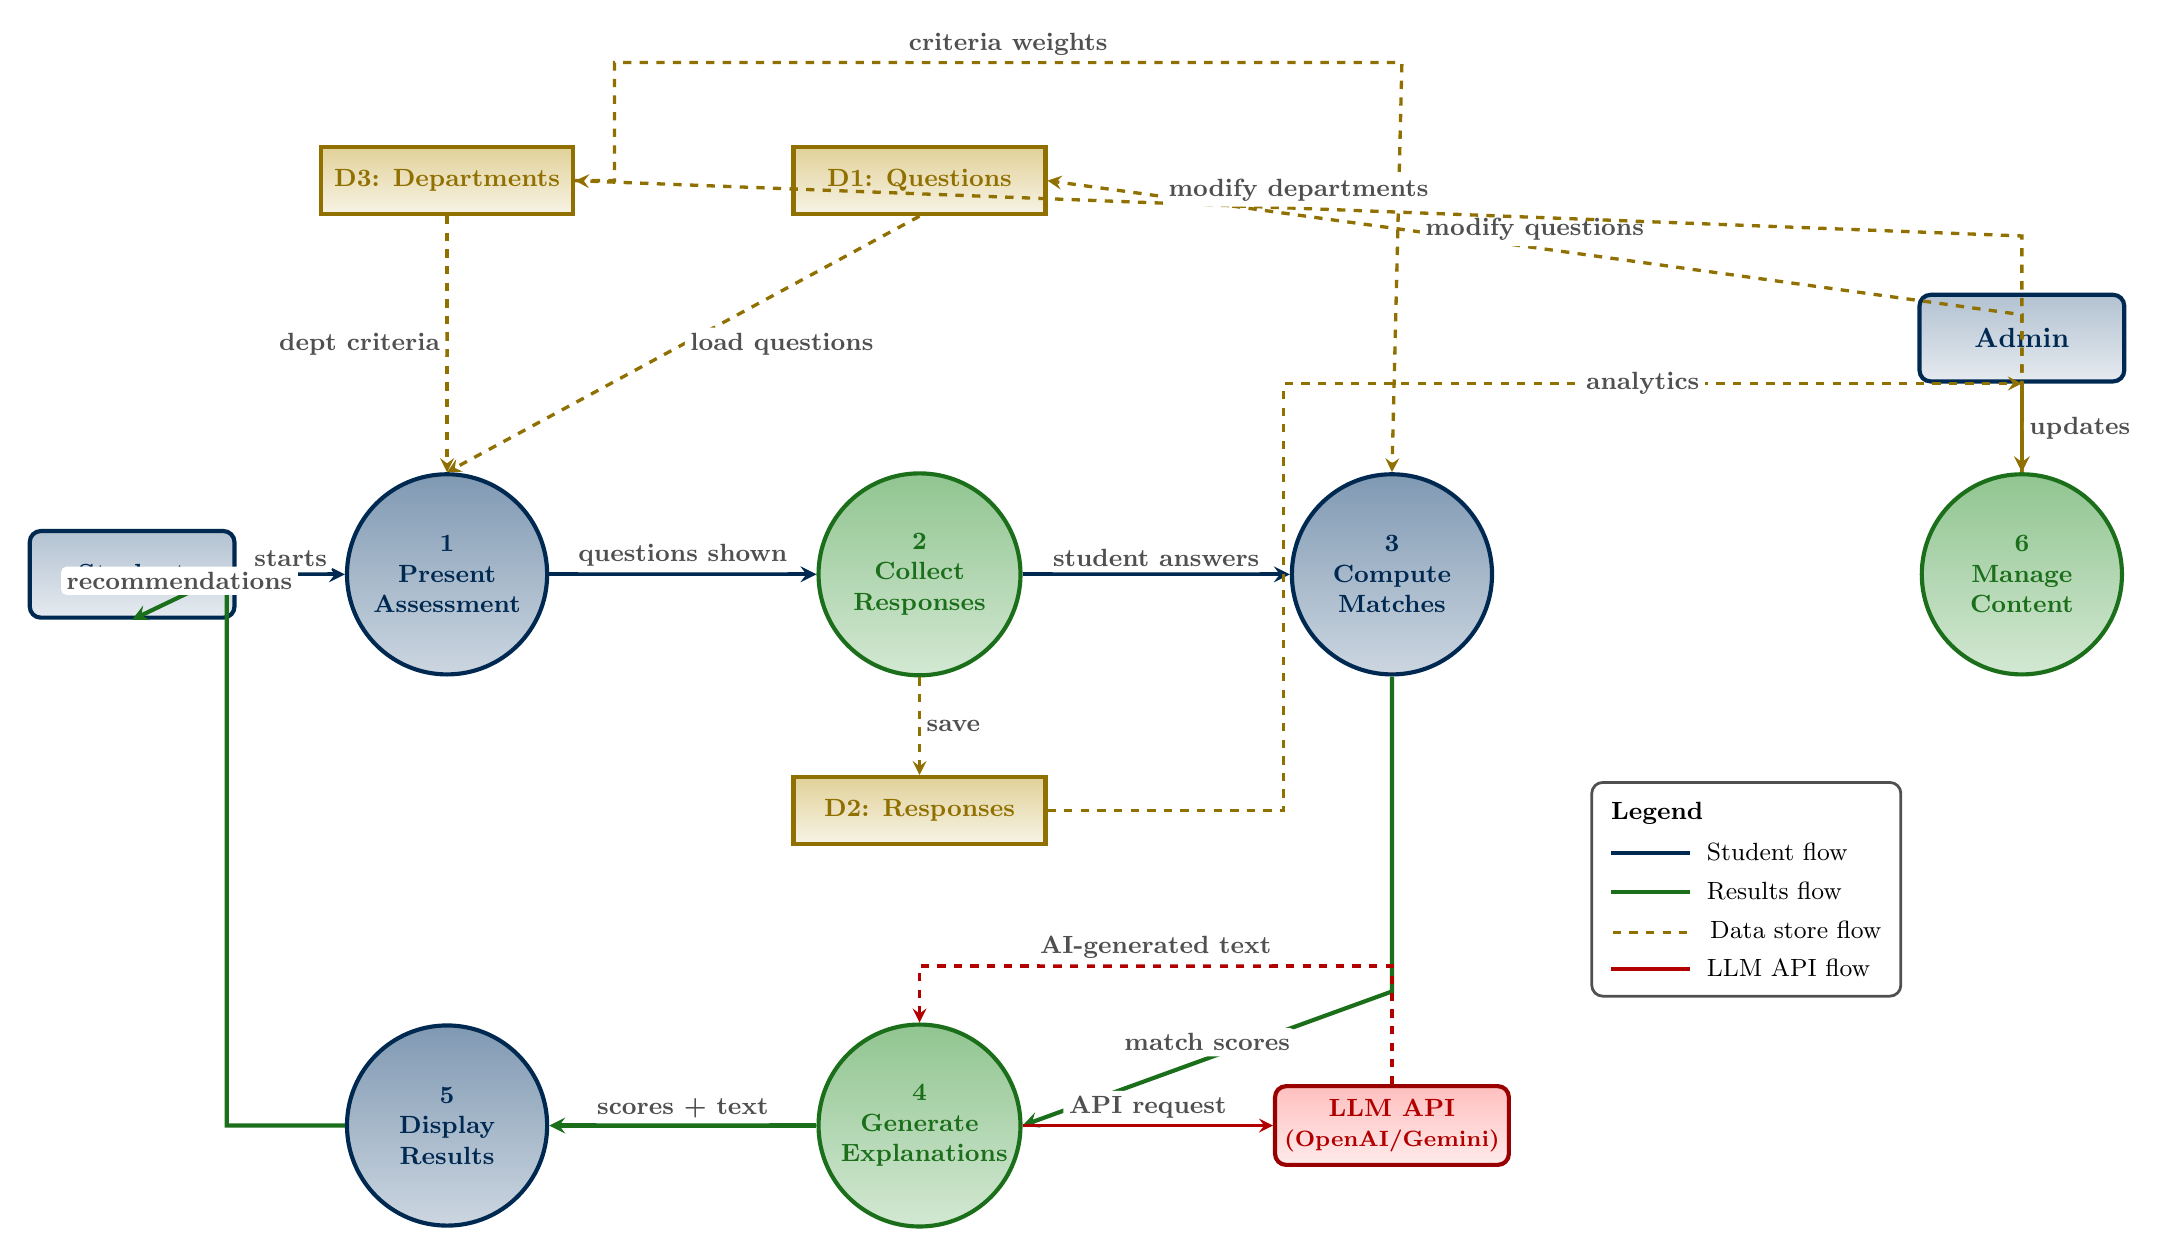
\begin{tikzpicture}[x=1cm, y=1cm]
\tikzset{
  entity/.style={rectangle, rounded corners=4pt, draw=uniblue!80!black, line width=1.5pt,
    top color=uniblue!30, bottom color=uniblue!10,
    minimum width=2.6cm, minimum height=1.1cm, align=center, font=\normalsize\bfseries, text=uniblue!80!black},
  procblue/.style={circle, draw=uniblue!80!black, line width=1.5pt,
    top color=uniblue!50, bottom color=uniblue!20, minimum size=2.4cm, align=center,
    font=\small\bfseries, text=uniblue!80!black},
  procgreen/.style={circle, draw=unigreen!80!black, line width=1.5pt,
    top color=unigreen!50, bottom color=unigreen!20, minimum size=2.4cm, align=center,
    font=\small\bfseries, text=unigreen!80!black},
  datastore/.style={rectangle, draw=accentgold!80!black, line width=1.5pt,
    top color=accentgold!40, bottom color=accentgold!10,
    minimum width=3.2cm, minimum height=0.85cm, align=center,
    font=\small\bfseries, text=accentgold!80!black},
  extapi/.style={rectangle, rounded corners=4pt, draw=red!60!black, line width=1.5pt,
    top color=red!25, bottom color=red!8, minimum width=2.6cm, minimum height=1cm,
    align=center, font=\small\bfseries, text=red!70!black},
  fl/.style={->, line width=1.2pt, >=stealth},
  lbl/.style={font=\small\bfseries, fill=white, inner sep=2pt, rounded corners=2pt, text=darkgray}
}
\node[entity]  (student) at (0,   8)  {Student};
\node[entity]  (admin)   at (24,  11) {Admin};
\node[extapi]  (llm)     at (16,  1)  {LLM API\\{\footnotesize(OpenAI/Gemini)}};
\node[datastore] (d3) at (4,  13) {D3: Departments};
\node[datastore] (d1) at (10, 13) {D1: Questions};
\node[datastore] (d2) at (10, 5)  {D2: Responses};
\node[procblue,  text width=2cm] (p1) at (4,  8)  {\textbf{1}\\Present\\Assessment};
\node[procgreen, text width=2cm] (p2) at (10, 8)  {\textbf{2}\\Collect\\Responses};
\node[procblue,  text width=2cm] (p3) at (16, 8)  {\textbf{3}\\Compute\\Matches};
\node[procgreen, text width=2cm] (p4) at (10, 1)  {\textbf{4}\\Generate\\Explanations};
\node[procblue,  text width=2cm] (p5) at (4,  1)  {\textbf{5}\\Display\\Results};
\node[procgreen, text width=2cm] (p6) at (24, 8)  {\textbf{6}\\Manage\\Content};
\draw[fl, color=uniblue!80!black, line width=1.5pt] (student) -- node[lbl,above] {starts} (p1);
\draw[fl, color=uniblue!80!black, line width=1.5pt] (p1) -- node[lbl,above] {questions shown} (p2);
\draw[fl, color=uniblue!80!black, line width=1.5pt] (p2) -- node[lbl,above] {student answers} (p3);
\draw[fl, color=accentgold!80!black, dashed, line width=1.2pt] (d1.south) -- node[lbl,right] {load questions} (p1.north);
\draw[fl, color=accentgold!80!black, dashed, line width=1.2pt] (d3.south) -- node[lbl,left] {dept criteria} (p1.north);
\draw[fl, color=accentgold!80!black, dashed, line width=1.2pt] (d3.east) -- ++(0.5,0) -- ++(0,1.5) -- node[lbl,above] {criteria weights} ++(10,0) -- (p3.north);
\draw[fl, color=accentgold!80!black, dashed, line width=1.2pt] (p2.south) -- node[lbl,right] {save} (d2.north);
\draw[fl, color=unigreen!80!black, line width=1.5pt] (p3.south) -- ++(0,-4) -- node[lbl,above] {match scores} (p4.east);
\draw[fl, color=unigreen!80!black, line width=1.5pt] (p4) -- node[lbl,above] {scores + text} (p5);
\draw[fl, color=unigreen!80!black, line width=1.5pt] (p5.west) -- ++(-1.5,0) -- ++(0,7) -- node[lbl,above] {recommendations} (student.south);
\draw[fl, color=red!70!black, line width=1.2pt] (p4.east) -- node[lbl,above] {API request} (llm.west);
\draw[fl, color=red!70!black, dashed, line width=1.2pt] (llm.north) -- ++(0,1.5) -- node[lbl,above] {AI-generated text} ++(-6,0) -- (p4.north);
\draw[fl, color=accentgold!80!black, line width=1.5pt] (admin) -- node[lbl,right] {updates} (p6);
\draw[fl, color=accentgold!80!black, dashed, line width=1.2pt] (p6.north) -- ++(0,2) -- node[lbl,above] {modify questions} (d1.east);
\draw[fl, color=accentgold!80!black, dashed, line width=1.2pt] (p6.north) -- ++(0,3) -- node[lbl,above] {modify departments} (d3.east);
\draw[fl, color=accentgold!80!black, dashed, line width=1.2pt] (d2.east) -- ++(3,0) |- node[lbl,right,pos=0.7] {analytics} (admin.south);
\node[draw=darkgray, fill=white, rounded corners=4pt, inner sep=7pt, font=\small, align=left, line width=1pt] at (20.5, 4) {
  \textbf{Legend}\\[4pt]
  {\color{uniblue!80!black}\rule[2pt]{1cm}{1.5pt}}\ \ Student flow\\[3pt]
  {\color{unigreen!80!black}\rule[2pt]{1cm}{1.5pt}}\ \ Results flow\\[3pt]
  {\color{accentgold!80!black}\tikz[baseline=-0.5ex]\draw[dashed,line width=1.2pt,color=accentgold!80!black](0,0)--(1,0);}\ \ Data store flow\\[3pt]
  {\color{red!70!black}\rule[2pt]{1cm}{1.5pt}}\ \ LLM API flow
};
\end{tikzpicture}%
}
\caption{Level 1 DFD --- major processes and data stores}
\end{figure}

\paragraph{Level 2 DFD (Process 3 Decomposition)}

\begin{figure}[H]
\centering
\resizebox{\textwidth}{!}{%
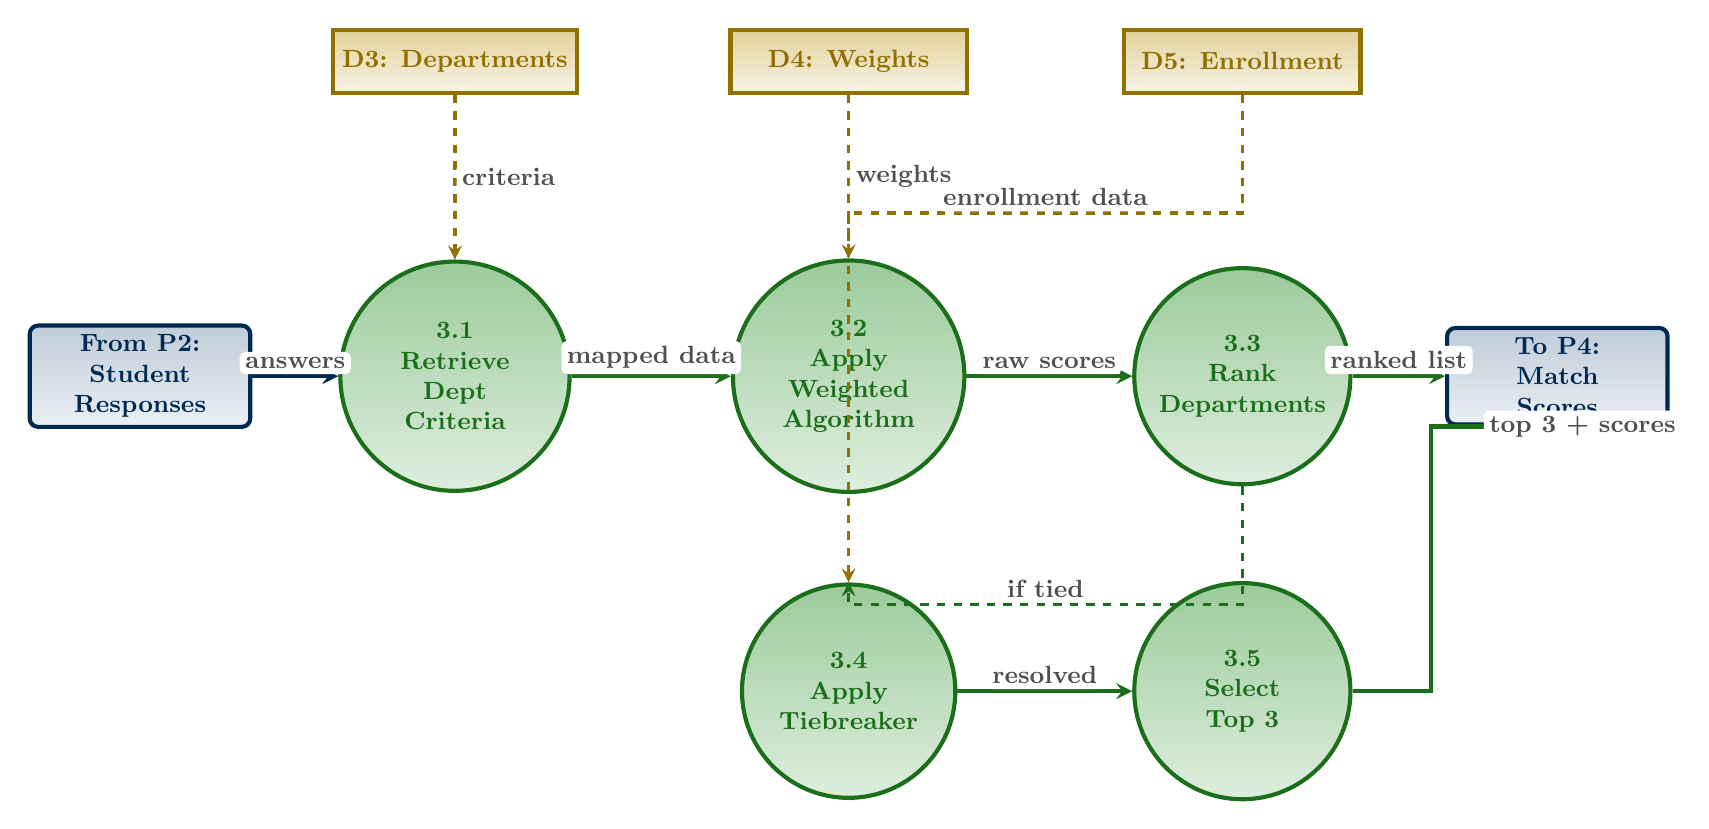
\begin{tikzpicture}[x=1cm, y=1cm]
\tikzset{
  proc2/.style={circle, draw=unigreen!80!black, line width=1.5pt,
    top color=unigreen!45, bottom color=unigreen!15,
    minimum size=2.4cm, align=center, font=\small\bfseries, text=unigreen!80!black},
  ds2/.style={rectangle, draw=accentgold!80!black, line width=1.5pt,
    top color=accentgold!40, bottom color=accentgold!10,
    minimum width=3cm, minimum height=0.8cm, align=center, font=\small\bfseries, text=accentgold!80!black},
  extbox/.style={rectangle, rounded corners=3pt, draw=uniblue!80!black, line width=1.5pt,
    top color=uniblue!25, bottom color=uniblue!08,
    minimum width=2.8cm, minimum height=1cm, align=center, font=\small\bfseries, text=uniblue!80!black},
  fl2/.style={->, line width=1.2pt, >=stealth, darkgray},
  lbl2/.style={font=\small\bfseries, fill=white, inner sep=2pt, rounded corners=2pt, text=darkgray}
}
\node[extbox] (input)  at (0,  5) {From P2:\\Student\\Responses};
\node[extbox] (output) at (18, 5) {To P4:\\Match\\Scores};
\node[ds2] (d3) at (4,  9) {D3: Departments};
\node[ds2] (d4) at (9,  9) {D4: Weights};
\node[ds2] (d5) at (14, 9) {D5: Enrollment};
\node[proc2, text width=2.2cm] (p31) at (4,  5) {\textbf{3.1}\\Retrieve\\Dept Criteria};
\node[proc2, text width=2.2cm] (p32) at (9,  5) {\textbf{3.2}\\Apply Weighted\\Algorithm};
\node[proc2, text width=2.2cm] (p33) at (14, 5) {\textbf{3.3}\\Rank\\Departments};
\node[proc2, text width=2.2cm] (p34) at (9,  1) {\textbf{3.4}\\Apply\\Tiebreaker};
\node[proc2, text width=2.2cm] (p35) at (14, 1) {\textbf{3.5}\\Select\\Top 3};
\draw[fl2, color=uniblue!80!black, line width=1.5pt] (input) -- node[lbl2,above] {answers} (p31);
\draw[fl2, color=unigreen!80!black, line width=1.5pt] (p31) -- node[lbl2,above] {mapped data} (p32);
\draw[fl2, color=unigreen!80!black, line width=1.5pt] (p32) -- node[lbl2,above] {raw scores} (p33);
\draw[fl2, color=unigreen!80!black, line width=1.5pt] (p33) -- node[lbl2,above] {ranked list} (output);
\draw[fl2, color=accentgold!80!black, dashed] (d3.south) -- node[lbl2,right] {criteria} (p31.north);
\draw[fl2, color=accentgold!80!black, dashed] (d4.south) -- node[lbl2,right] {weights} (p32.north);
\draw[fl2, color=accentgold!80!black, dashed] (d5.south) -- ++(0,-1.5) -- node[lbl2,above] {enrollment data} ++(-5,0) -- (p34.north);
\draw[fl2, color=unigreen!80!black, dashed] (p33.south) -- ++(0,-1.5) -- node[lbl2,above] {if tied} ++(-5,0) -- (p34.north);
\draw[fl2, color=unigreen!80!black, line width=1.5pt] (p34) -- node[lbl2,above] {resolved} (p35);
\draw[fl2, color=unigreen!80!black, line width=1.5pt] (p35.east) -- ++(1,0) |- node[lbl2,right,pos=0.7] {top 3 + scores} (output.south);
\end{tikzpicture}%
}
\caption{Level 2 DFD --- decomposition of Process 3 (Compute Matches)}
\end{figure}

% ─────────────────────────────────────────────────────────────────────────────
\subsection{User Interface Design}
% ─────────────────────────────────────────────────────────────────────────────



\subsubsection*{Navigational Flow}



% ─────────────────────────────────────────────────────────────────────────────
\subsection{Software Architecture}
% ─────────────────────────────────────────────────────────────────────────────

The system follows a \textbf{three-tier architecture} (Presentation, Application Logic, Data) deployed across free-tier cloud services.

\subsubsection*{Architecture Overview}



\subsubsection*{Subsystem Decomposition}

\begin{itemize}[leftmargin=1.5em, itemsep=3pt]
    \item \textbf{Assessment Module}: Renders questions, tracks progress, validates responses, auto-saves to localStorage
    \item \textbf{Recommendation Engine}: Weighted scoring algorithm, tiebreaker logic, top-3 selection
    \item \textbf{LLM Integration Module}: API wrapper with prompt templating, 5-second timeout, caching, template fallback
    \item \textbf{Department Repository}: CRUD operations for department profiles, content versioning
    \item \textbf{Admin Dashboard}: Authentication, content editor, analytics charts, CSV export
    \item \textbf{API Layer}: RESTful Express routes, input validation (express-validator), error handling middleware
\end{itemize}

\subsubsection*{Database Schema (Key Collections)}

\begin{table}[H]
\centering
\begin{tabularx}{\textwidth}{p{3cm}Xp{2.5cm}}
\toprule
\theadrow
\textbf{Collection} & \textbf{Key Fields} & \textbf{Retention} \\
\midrule
\texttt{departments}  & \_id, name, coreFocus, differentiators, curriculum, careerOutcomes, misconceptions, criteriaWeights\{\}, lastUpdated & Permanent \\[4pt]
\rowalt
\texttt{questions}    & \_id, text, responseOptions[], departmentWeights\{\}, category, order, isActive & Permanent \\[4pt]
\texttt{sessions}     & \_id, sessionId, responses[], matchScores\{\}, topRecommendations[], completedAt, feedback & 30 days \\[4pt]
\rowalt
\texttt{adminUsers}   & \_id, username, passwordHash, role, lastLogin & Permanent \\[4pt]
\texttt{analytics}    & \_id, date, completions, departmentDistribution\{\}, avgScores\{\} & Permanent (aggregated) \\
\bottomrule
\end{tabularx}
\caption{MongoDB collection schema summary}
\end{table}

% ─────────────────────────────────────────────────────────────────────────────
\subsection{Security and Access Control}
% ─────────────────────────────────────────────────────────────────────────────

\subsubsection*{Authentication}

\begin{itemize}[leftmargin=1.5em, itemsep=3pt]
    \item \textbf{Admin login}: Username + password; passwords hashed with bcrypt (cost factor 12); session managed via JSON Web Token (JWT) with 30-minute expiry
    \item \textbf{Student access}: No authentication required; system operates in anonymous mode to maximize adoption
    \item \textbf{Session security}: JWT stored in httpOnly cookie to prevent XSS attacks; CSRF protection via SameSite cookie attribute
\end{itemize}

\subsubsection*{Authorization}

\begin{table}[H]
\centering
\small
\begin{tabularx}{\textwidth}{>{\raggedright\arraybackslash}p{2.8cm}>{\raggedright\arraybackslash}p{3.2cm}>{\raggedright\arraybackslash}X>{\raggedright\arraybackslash}p{3.5cm}}
\toprule
\theadrow
\textbf{Role} & \textbf{Resource} & \textbf{Permitted Actions} & \textbf{Restricted Actions} \\
\midrule
Student (anon) & Assessment, Results, Comparison & Read questions, submit responses, view recommendations, download PDF & Modify content, view analytics \\[6pt]
\rowalt
Admin          & All resources & Full CRUD on departments, questions; view analytics; export CSV; manage users & \textit{(none)} \\[6pt]
HOD (future)   & Department profiles & Update own department profile only & Modify other departments, view analytics \\[6pt]
\bottomrule
\end{tabularx}
\caption{Role-based access control matrix}
\label{tab:rbac}
\end{table}

\vspace{8pt}

\subsubsection*{Data Privacy and Encryption}

\begin{itemize}[leftmargin=1.5em, itemsep=3pt]
    \item All communication between client, server, and database uses \textbf{HTTPS/TLS}
    \item Student responses stored without any personal identifiers (no name, email, or student ID collected)
    \item Response data automatically deleted after 30 days via a scheduled MongoDB TTL index
    \item Aggregated analytics data stripped of any individually identifiable patterns before storage
\end{itemize}

\clearpage

% ══════════════════════════════════════════════════════════════════════════════
%  CHAPTER 5: IMPLEMENTATION
% ══════════════════════════════════════════════════════════════════════════════
\section{Implementation}

\begin{tcolorbox}[enhanced, colback=accentgold!10, colframe=accentgold, arc=3pt, boxrule=1pt, top=6pt, bottom=6pt]
\textbf{Note:} This chapter documents the actual implementation. Fill in each section with your real development experience, screenshots, and test results.
\end{tcolorbox}

% ─────────────────────────────────────────────────────────────────────────────
\subsection{Development Process}
% ─────────────────────────────────────────────────────────────────────────────



\subsubsection*{Tools Used in Development}



% ─────────────────────────────────────────────────────────────────────────────
\subsection{Challenges and Solutions}
% ─────────────────────────────────────────────────────────────────────────────



% ─────────────────────────────────────────────────────────────────────────────
\subsection{Testing}
% ─────────────────────────────────────────────────────────────────────────────

\subsubsection*{Unit Testing}



\subsubsection*{Integration Testing}



\subsubsection*{System / User Acceptance Testing}



\subsubsection*{Performance Testing}



\clearpage

% ══════════════════════════════════════════════════════════════════════════════
%  CHAPTER 6: INTERNSHIP REFLECTION AND CONCLUSION
% ══════════════════════════════════════════════════════════════════════════════
\section{Internship Reflection and Conclusion}

\begin{tcolorbox}[enhanced, colback=accentgold!10, colframe=accentgold, arc=3pt, boxrule=1pt, top=6pt, bottom=6pt]
\textbf{Note:} This chapter is personal and requires your genuine reflection. Write in first person (or ``we'' for group experiences). Be honest and specific --- use real examples from your internship experience.
\end{tcolorbox}

% ─────────────────────────────────────────────────────────────────────────────
\subsection{Learning Outcomes}
% ─────────────────────────────────────────────────────────────────────────────



% ─────────────────────────────────────────────────────────────────────────────
\subsection{Challenges Faced}
% ─────────────────────────────────────────────────────────────────────────────



% ─────────────────────────────────────────────────────────────────────────────
\subsection{Recommendations}
% ─────────────────────────────────────────────────────────────────────────────

\subsubsection*{Recommendations for the Host Organization (ICT Center / CCI)}



\subsubsection*{Recommendations for Future Internship Programs}



\clearpage

% ══════════════════════════════════════════════════════════════════════════════
%  APPENDICES
% ══════════════════════════════════════════════════════════════════════════════
\appendix
\renewcommand{\thesection}{\Alph{section}}

\section{Student Survey Questionnaire}
\label{appendix:survey}



\section{HOD Interview / Questionnaire Template}
\label{appendix:hod}



\section{Selected Code Snippets}
\label{appendix:code}



\section{Full DFD Diagrams (Large Format)}
\label{appendix:dfds}



% ══════════════════════════════════════════════════════════════════════════════
%  REFERENCES
% ══════════════════════════════════════════════════════════════════════════════
\clearpage
\section*{References}
\addcontentsline{toc}{section}{References}



\begin{enumerate}[label={[\arabic*]}, leftmargin=2.5em, itemsep=4pt]
    \item 
    \item 
    \item 
\end{enumerate}

% ══════════════════════════════════════════════════════════════════════════════
\end{document}
% ══════════════════════════════════════════════════════════════════════════════
